\chapter{Sviluppo del modulo nfproxy}

Come già esplicitato in prcedenza, il regex filtering è un modello di filtraggio che permette si ottime prestazioni (pochè processato, e costruito con linguaggi
e librerie veloci e low level), ma presentava delle grandi limitazioni in termini di flessibilità nell'analisi delle richieste e delle risposte, anche considerando che
la maggior parte dei servizi in ambito CTF girano su protocolli quali HTTP o a spesso unicamente su canali TCP, per esporre interfacce di programmi da terminale,
che spesso hanno parte dei loro contenuti compressi o rappresentati tramite encoding i quali contenuti non sono facilmente analizzabili tramite regex. \\

Al costo di prestazioni inferiori, con il vantaggio di poter scrivere i filtri in un linguaggio di semplice utilizzo e rapido per lo scripting quale
\texttt{Python}\footcite{\url{http://python.org/}}{python}, \texttt{nfproxy} è stato sviluppato proprio ai fin di superare i precedenti limiti lasciando una
estesa libertà nell'implementazione delle logiche di filtraggio del traffico,
mantenendo comunque un ottimo livello di prestazioni grazie ad alcune scelte architetturali intraprese e a diversi strumenti di sviluppo descritti in seguito.\\

\texttt{Nfproxy} non è propriamente di per se un proxy, ma un modulo che sfrutta l'utilizzo di
\texttt{nfqueue}\footcite{\url{https://netfilter.org/projects/libnetfilter_queue/}}{netfilter_queue} lasciando un grado di controllo sul traffico e una facilità di utilizzo
paragonabili a quella di un tradizionale proxy, dando in aggiunta accesso diretto ai pacchetti a livello di rete e inoltre non presenta le problematiche di
cambio di configurazione del servizio originale per applicare i filtri, poichè il traffico viene intercettato in
maniera totalmente invisibile, non richiedendo pertanto alcuna modifica sull'applicativo.\\
Si noti tuttavia come questa implementazione presenti alcune limitazioni riguardo la modifica, che però non rappresentano un scenario di utilizzo necessario
e strettamente utile per la difesa stessa del servizio. La parte che gestisce la queue come vedremo in seguito, è sviluppata tramite un utilizzo ibrido
di \texttt{C++} e \texttt{Python}, al fine di sfruttare alcune caratteristiche e librerie di \texttt{C++} per la gestione dei pacchetti, e permettere
l'utilizzo di python per il parsing ed il filtraggio dei pacchetti.
Il modulo supporta nativamente il parsing di HTTP/1.1\footcite{RFC2616, Hypertext Transfer Protocol -- HTTP/1.1}{rfc2616}, Websocket\footcite{RFC6455, The WebSocket Protocol}{rfc6455} e del normale flusso TCP\footcite{RFC9293, Transmission Control Protocol (TCP)}{rfc9293}.

\section{Requisiti}

Di seguito si elencano i requisiti principali, obiettivi dello sviluppo del seguente modulo:

\begin{itemize}
    \setlength{\itemsep}{5pt}
    \setlength{\parskip}{5pt}
    \item \texttt{Utilizzo del linguaggio python per la scrittura dei filtri}: il modulo deve offrire come strumenti di sviluppo dei filtri
    il linguaggio python, tramite l'ausilio di funzionalità offerte dal modulo stesso, ottimali, semplici per l'utilizzo per la scrittura dei filtri.
    \item \texttt{Supporto ai protocolli HTTP/1.1 e Websocket}: il modulo deve supportare nativamente il parsing dei pacchetti HTTP/1.1 e Websocket eseguendone il parsing
    e rendendo disponibili i dati già decodificati e decodificati quando è possibile, garantendone un accesso immediato. Deve supportare pertando i metodi di decompressione
    quali \texttt{gzip}\footcite{RFC1952, GZIP file format specification version 4.3}{rfc1952},
    \texttt{deflate}\footcite{RFC1951, DEFLATE Compressed Data Format Specification version 1.3}{rfc1951},
    \texttt{brotli}\footcite{RFC7932, Brotli Compressed Data Format}{rfc7932},
    \texttt{zstd}\footcite{RFC8478, Zstandard Compression and the application/zstd Media Type}{rfc8478}.
    Deve supportare anche l'estensione per websocket \texttt{permessage-deflate}\footcite{RFC7692, Compression Extensions for WebSocket}{rfc7692}.
    \item \texttt{Supporto al parsing dei pacchetti TCP}: il modulo deve supportare il parsing dei pacchetti TCP, permettendo l'accesso ai dati di livello di trasporto con payload già ordinati.
    \item \texttt{Accesso agli header ai livelli di rete e di trasporto}: il modulo deve permettere degli header IP e TCP accessibili e modificabili.
    \item \texttt{Supporto a IPv4 e IPv6}: il modulo deve supportare il parsing dei pacchetti IPv4\footcite{RFC791, Internet Protocol}{rfc791} e IPv6\footcite{RFC2460, Internet Protocol, Version 6 (IPv6) Specification}{rfc2460}.
    \item \texttt{Gestione autonoma dei buffer}: il modulo deve gestire autonomamente i buffer di memoria, evitando di sovraccaricare la memoria del sistema e di
    delegare la gestione di questi al programmatore, tuttavia lasciando la libertà di decisione sulle modalità di gestione, fornendo delle opzioni di configurazione opzionali.
    \item \texttt{Segnalazione degli errori}: il modulo deve segnalare in maniera chiara e precisa gli errori di parsing e di esecuzione dei filtri, facendo noto 
    al programmatore errori inaspettati rilevati e fornendo i log necessari per la risoluzione.
    \item \texttt{Supporto alla gestione dei filtri in maniera immediata}: deve essere possibile disabilitare totalmente o parzialmente i filtri in maniera immediata e
    senza downtime del servizio.
    \item \texttt{Supporto alla paralelizzazione}: il modulo deve supportare la paralelizzazione dei pacchetti, permettendo di sfruttare al meglio le risorse del sistema
    e garantendo un'ottima scalabilità del firewall.
    \item \texttt{Possibilitò di verifica del filtro tramite simulazione}: il modulo deve permettere di verificare il filtro in maniera simulata, permettendo di testare
    il quest'ultimo senza dover necessariamente applicarlo direttamente al traffico della macchina, permettendone il debugging e lo sviluppo in modo sicuro e rapido.
  \end{itemize}

\section{Architettura}

Il modulo nfproxy è avviato dal backend di firegex, che si occupa a sua volta di impostare le regole di \texttt{nftables}\footcite{\url{https://netfilter.org/projects/nftables/}}{nftables} tramite le sue API json,
avviare il modulo c++ dove viene gestita tutta la logica principale di multithreading, gestione dei pacchetti, assemblaggio dei payload
TCP e parsing del livello applicativo ed infine alla applicazione dei filtri python.\\
Di seguito un diagramma dell'architettura del modulo nfproxy, le varie componenti verranno analizzate nel dettaglio in seguito:

\begin{figure}[H]
    \centering
    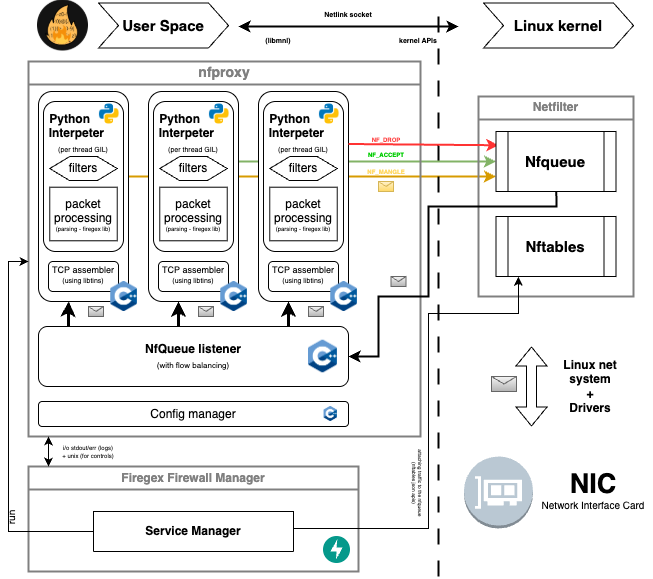
\includegraphics[width=0.9\textwidth]{images/chapter3/nfproxy.drawio.png}
    \caption{Architettura del modulo nfqueue}
    \label{fig:firegex_arch}
\end{figure}

\section{Elaborazione parallelizzata dei pacchetti}

Uno dei principali ostacoli affrontati durante la progettazione è stata proprio la gestione della parallelizzazione dei processi di elaborazione, 
a causa di una serie di problematiche descritte in seguito riguardo il funzionamento di \texttt{nfqueue}, alcune caratteristiche il linguaggio
python, e anche la necessità di far interfacciare 2 linguaggi differenti in un unico modulo.\\
Obiettivi principali della paralellizzazione sono stati:
\begin{itemize}
    \setlength{\itemsep}{5pt}
    \setlength{\parskip}{5pt}
    \item \texttt{Evitare la possibilità di conflitti di dati tra i processi}: Elemento critico nella progettazione per cui si devono evitare quanto possibile i conflitti
    tra i vari processi di modo da evitare corruzione di dati, crash improvvisi e comportamenti inaspettati.
    \item \texttt{Evitare l'utilizzo di elementi bloccanti quali le lock}: i lock spesso ricorrono utili nella gestione di risorse condivise, ma possono portare a problemi
    di prestazioni e di deadlock: pertanto uno degli obiettivi fissati è ridurre il loro utilizzo al minimo indispensabile, strutturando il sistema appositamente per eviatre 
    casistiche in cui è necessario il loro utilizzo.
    \item \texttt{Evitare copie in memoria, e avvio di processi sovrabbondanti}: Evitando le copie in memoria dei pacchetti, riduciamo il
    consumo di memoria ma soprattutto velociziamo il processo di analisi garantendo maggiori performance.
\end{itemize}
Per le motivazioni sopra citate, si è scelto un approccio alla parallelizzazione di tipo produttore-consumatore, che vede come produttore
un processo ascoltatore, che riceve dal kernel i pacchetti da elaborare, il quale fa effettivamente il binding della \texttt{nfqueue},
e diversi processi consumatori che hanno come uniche risorse comuni delle dequeue di pacchetti, che verranno distribuiti dal produttore.
Il produttore quindi accoderà i pacchetti in queste code, che verranno prevelati dai relativi consumatori per essere elaborati.
Il singolo consumatore si occupa di ordinare i pacchetti TCP, elaborare i filtri python, ed infine mandare i
\texttt{verdicts}\footcite{\url{https://netfilter.org/projects/libnetfilter_queue/doxygen/html/group__nfq__verd.html}}{vedicts_nfqueue}
al kernel per eseguire l'azione richiesta sul pacchetto, e procedere con la prossima elaborazione.\\
Per ogni consumatore ci sarà una coda di pacchetti separata condivisa unicamente con il produttore, la quale sarà l'unico elemento critico in cui verranno utilizzate le lock.\\
Si specifica che si è pensato anche ad una scelta implementativa diversa per le dequeue tramite l'utilizzo delle \texttt{unix pipe}\footcite{\url{https://man7.org/linux/man-pages/man2/pipe.2.html}}{unix_pipe},
tuttavia si è scelto di utilizzare un'implementazione che fa utilizzo di \texttt{std::mutex}\footcite{\url{https://en.cppreference.com/w/cpp/thread/mutex}}{std_mutex} e
\texttt{std::condition\_variable}\footcite{\url{https://en.cppreference.com/w/cpp/thread/condition_variable}}{condition_variable_std} per ragioni di performance
e di possibilità di implementare un sistema di blocco della coda in push in caso di riempimento che ferma il processo produttore (evitando di riempire eccessivamente queste code).
L'implementazione utilizzata è stata quella di \texttt{Arif Jaffer}\footcite{\url{https://www.bit-byter.com/blog/files/blocking-q-cpp.html}}{blocking_queue_cpp}.

\subsection{A Per-Interpreter GIL con python 3.12}

Una delle problematiche citate precedentemente sulla paralelizzazione erano riguardo una caratteristica del linguaggio python,
il \texttt{GIL}\footcite{Understanding the python gil}{beazley2010understanding} (Global Interpeter Lock), che limita l'utilizzo dei thread in python
permettendo ad un solo thread per volta l'esecuzione del codice, che altrimenti presenterebbe problemi riguardo la gestione degli oggetti python stessi
poichè internamente (come ad esempio per il sistema di reference counting) la loro gestione non è implementata in maniera thread-safe e incorrerebbe a comportamenti inaspettati.\\
Inoltre si sottlinea come python in questa casistica gestisce unicamente operazioni CPU-bound, che vanno ulteriormente ad evidenziare gli svantaggi portati dal GIL.\\

\begin{figure}[H]
    \centering
    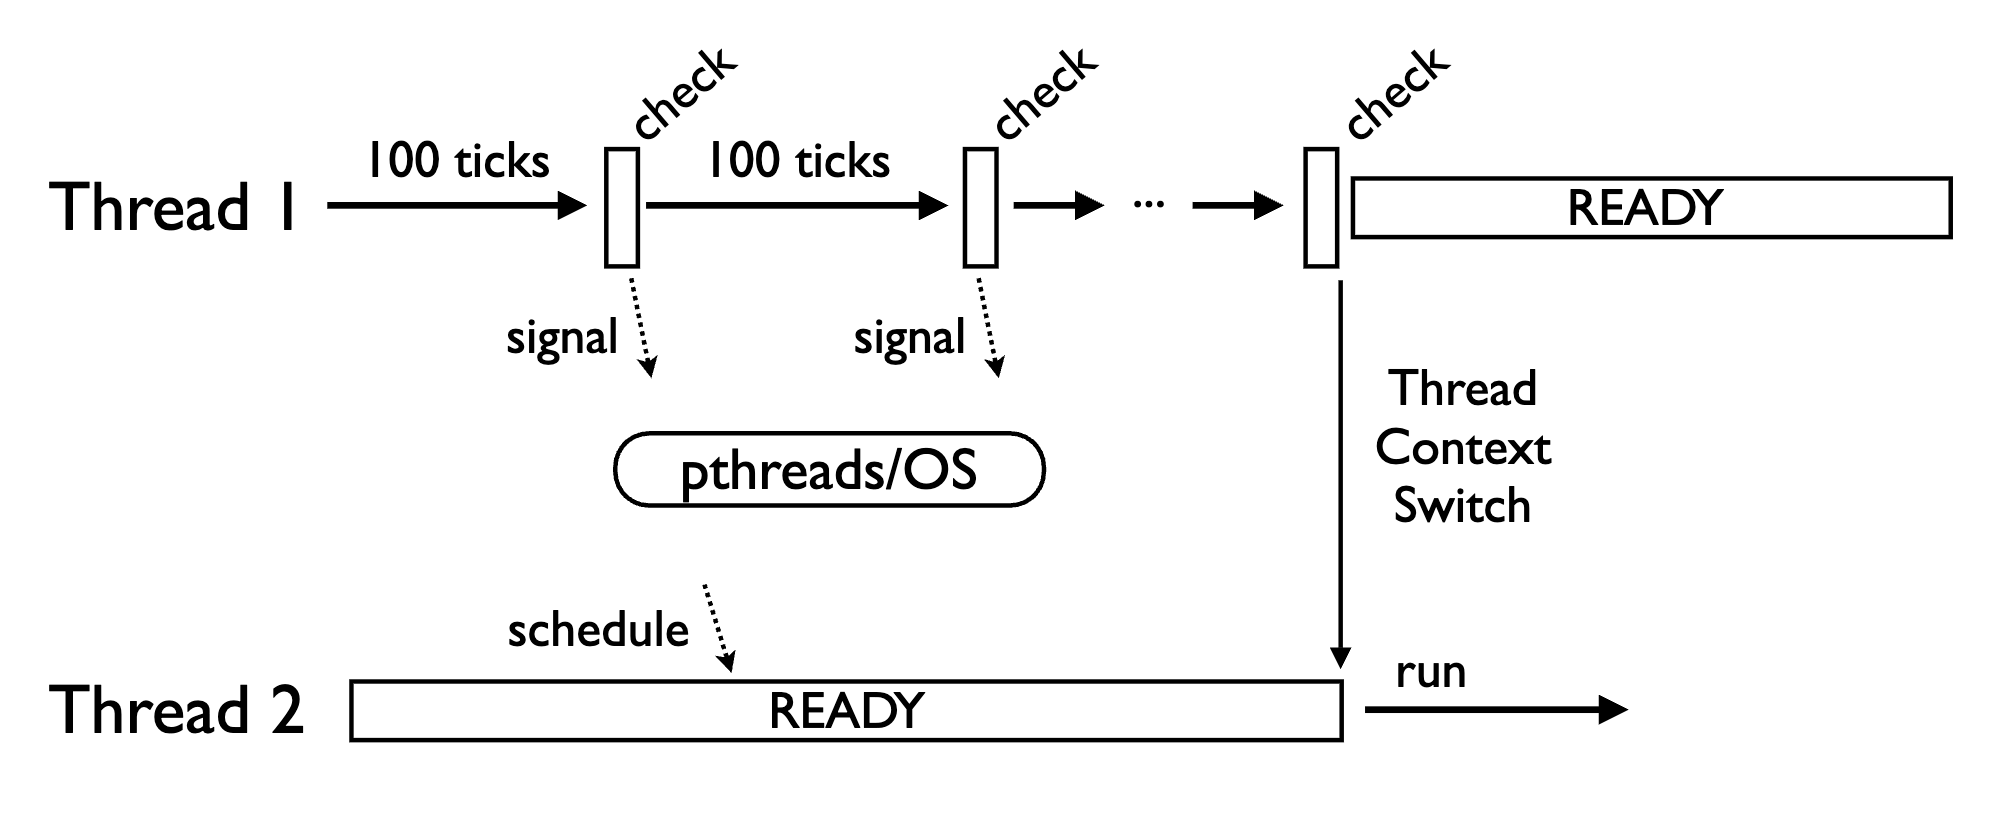
\includegraphics[width=0.8\textwidth]{images/chapter3/GIL.png}
    \caption{Python Global Interpeter Lock}
    \label{fig:py_gil_schema}
\end{figure}

Una soluzione potrebbe essere sarebbe quella di utilizzare processi multipli, che permettono di avere un GIL per ogni processo,
ma che porterebbe ad un overhead per la necessità di aggiuntivi inter-process communication con i nuovi processi, e di copia di elementi in memoria.\\

La soluzione adottata per questo problema è relativa ad una importante modifica in \texttt{Python 3.12} relativa al
\texttt{PEP 684}\footcite{\url{https://peps.python.org/pep-0684/}}{pep648}, che introduce la possibilità di avviare sullo stesso processo diversi interpreti python
ogniuno con il proprio GIL, permettendo l'esecizione di codice python in thread realmente parallelizzati.\\
L'utilizzo di questa funzionalità è unicamente accessibile tramite C-API, che ci permettono anche l'avvio diretto di un interprete python senza l'effettivo avvio dell'eseguibile
\texttt{python3}, ma direttamente tramite chiamate a \texttt{libpython}, permettendo anche alternare i 2 linguaggi facilmente.\\

Questo ha come limite il fatto che non è possibile condividere oggetti tra gli interpreti python, che però nella casistica corrente non è un problema, dato che non
ci sarà bisogno di condividere dati tra i thread, grazie al meccanismo di distribuzione dei pacchetti utilizzato descritto nel prossimo paragrafo che ne permette un completo isolamento.\\
Pertanto, una volta arrivata una nuova configurazione di filtri, alla prima nuova richiesta di elaborazione di un pacchetto, verrà ri-compilato il codice python (nel suo bytecode) e
serializzato tramite \texttt{marshal}\footcite{\url{https://docs.python.org/3/library/marshal.html}}{marshal_python} e verrà inizializzata per ogni connessione TCP
un nuovo contesto globale python che manterrà lo stato del filtro, e verrà distrutto alla fine della connessione.\\

L'implementazione di questa funzionalità tuttavia presenta i suoi limiti sul supporto di moduli python scritti con \texttt{cython}\footcite{\url{https://cython.org/}}{cython},
o in generale moduli che ad ora non sono stati tramite \texttt{multi-phase inizialization}\footcite{\url{https://peps.python.org/pep-0489/}}{pep489}, o che semplicemente hanno elementi che non sono
thread safe a loro interno. Questi moduli non possono essere utilizzati con questa implementazione, o possono portare a comportamenti inaspettati a causa di corruzioni di memoria.\\
Alcune problematiche riscontrate riguardo questo aspetto sono descritte successivamente.\\


\begin{listing}[H]
    \begin{minted}[
        frame=single,
        framerule=0.8pt,
        fontsize=\footnotesize,
        breaklines
      ]{cpp}
PyThreadState * tstate = nullptr;
PyObject* handle_packet_code = nullptr;
PyInterpreterConfig py_thread_config = {
    .use_main_obmalloc = 0,
    .allow_fork = 0,
    .allow_exec = 0,
    .allow_threads = 0,
    .allow_daemon_threads = 0,
    .check_multi_interp_extensions = 1,
    .gil = PyInterpreterConfig_OWN_GIL,
};

void before_loop() { // Function called on thread start
    PyStatus pystatus;
    // Creating a new thread state
    tstate = PyThreadState_New(PyInterpreterState_Main());
    // Acquire the GIL and switching with a new GIL
    PyEval_AcquireThread(tstate); 
    pystatus = Py_NewInterpreterFromConfig(&tstate, &py_thread_config);
    handle_packet_code = unmarshal_code(...); //Unmarshaling compiled code
    ...
}
\end{minted}
\end{listing}

Si evidenzia come una possibile soluzione alternativa a questa potrebbe essere stata utilizzare la versione priva di GIL di
\texttt{Python 3.13 free-threaded mode}\footcite{\url{https://docs.python.org/3/whatsnew/3.13.html\#whatsnew313-free-threaded-cpython}}{py13_free_threaded},
che tuttavia è stata rilasciata come feature sperimentale non consigliata per l'utilizzo in produzione, e per altro con un calo netto di performance a causa
del mancato supporto ad alcuni sistemi di ottimizzazione.

\subsection{Bilanciamento del carico}

Per il bilanciamento del carico sui processi consumatori che eseguiranno i filtri, al fine di isolare questi processi e garantire un'equa distribuzione
dei pacchetti, si è scelto di utilizzare un meccanismo basato su hashing su IP e porta sorgente e destinazione, che ne permettono un calcolo semplice e rapido
da eseguire e allo stesso tempo garantisce che gli stessi flussi di pacchetti vengano sempre elaborati dallo stesso processo consumatore, evitando quindi che
i vari consumatori debbano condividere risorse legate ai dati salvati riguardo quel specifico flusso.\\

\begin{listing}[H]
    \begin{minted}[
        frame=single,
        framerule=0.8pt,
        fontsize=\footnotesize,
        breaklines
      ]{cpp}
// Hash function for stream_id, valid for both IPv4 and IPv6
uint32_t hash_stream_id(const stream_id &sid) {
    uint32_t addr_hash = 0;
    addr_hash ^= min_addr[0] ^ min_addr[1] ^ min_addr[2] ^ min_addr[3];
    addr_hash ^= max_addr[0] ^ max_addr[1] ^ max_addr[2] ^ max_addr[3];
    uint32_t ports = (static_cast<uint32_t>(sid.min_address_port) << 16) | sid.max_address_port;
    uint32_t hash = addr_hash ^ ports;
    hash *= 0x9e3779b9; // More randomness (multiplication with a prime)
    return hash;
}

// Banacing function for the consumers (simplified)
void __real_handler(PktRequest<Worker>* pkt) {
    // Calculate the index of the consumer
    const size_t idx = hash_stream_id(pkt->sid) % pkt->ctx->size();
    // Put the packet in the queue
    converted_pkt->ctx->queue.put(converted_pkt);
}
\end{minted}
\end{listing}

Si sottolinea come una tecnica simile sia anche utilizzata direttamente kernel space per il bilanciamento del carico dei pacchetti.
La seguente gestione è stata fatta userspace e lasciata a nfqueue kernel space (come in una precedente implementazione usata per nfregex),
poichè l'hashing eseguito nel kernel per motivi tecnici legati alla generalizzazione del modulo per protocolli diversi da quelli di cui
si è interessati per lo sviluppo di nfproxy, nell'hashing eseguito lato kernel non viene utilizzata la porta.

\begin{listing}[H]
    \begin{minted}[
        frame=single,
        framerule=0.8pt,
        fontsize=\footnotesize,
        breaklines
      ]{cpp}
static inline u32
nfqueue_hash(const struct sk_buff *skb, u16 queue, u16 queues_total, u8 family,
	     u32 initval)
{
	switch (family) {
	case NFPROTO_IPV4:
		queue += reciprocal_scale(hash_v4(ip_hdr(skb), initval),
					  queues_total);
		break;
	case NFPROTO_IPV6:
		queue += reciprocal_scale(hash_v6(ipv6_hdr(skb), initval),
					  queues_total);
		break;
	case NFPROTO_BRIDGE:
		queue += reciprocal_scale(hash_bridge(skb, initval),
					  queues_total);
		break;
	}

	return queue;
}
\end{minted}
\end{listing}

Il codice precedentemente citato viene estrapolato direttamente dal kernel linux, e 
viene utilizzato nel bilanciamento di carico dei pacchetti\footnote{\url{https://web.git.kernel.org/pub/scm/linux/kernel/git/torvalds/linux.git/tree/net/netfilter/xt_NFQUEUE.c?h=v6.14-rc7\#n86}},
e il codice utilizzato per l'hashing\footnote{\url{https://web.git.kernel.org/pub/scm/linux/kernel/git/torvalds/linux.git/tree/include/net/netfilter/nf_queue.h?h=v6.14-rc7\#n105}}
come è possibile vedere non include la porta, che è stata aggiunta per il bilanciamento del carico in userspace.\\

Questo rappresenta un limite importante per l'utilizzo di questo modulo in contesti come le competizioni Attack Defence dove
troviamo traffico anonimizzato tramito l'ausilio di un NAT, che di per se pertanto porterebbe
ad un bilanciamento del carico non esistente poichè 1 solo consumatore verrebbe impegnato nell'elaborazione di tutti i pacchetti
se 1 solo ip è utilizzato nel NAT.\\
Di seguito si riporta un benchmark del modulo \texttt{nfregex} che utilizza il nuovo sistema di bilanciamento del carico userspace,
che simula del carico in elaborazione del traffico con il seguente codice:

\begin{listing}[H]
    \begin{minted}[
        frame=single,
        framerule=0.8pt,
        fontsize=\footnotesize,
        breaklines
      ]{cpp}
volatile int x = 0;
for (int i=0; i<50000; i++){
    x+=1;
}
\end{minted}
\end{listing}

\begin{figure}[H]
    \centering
    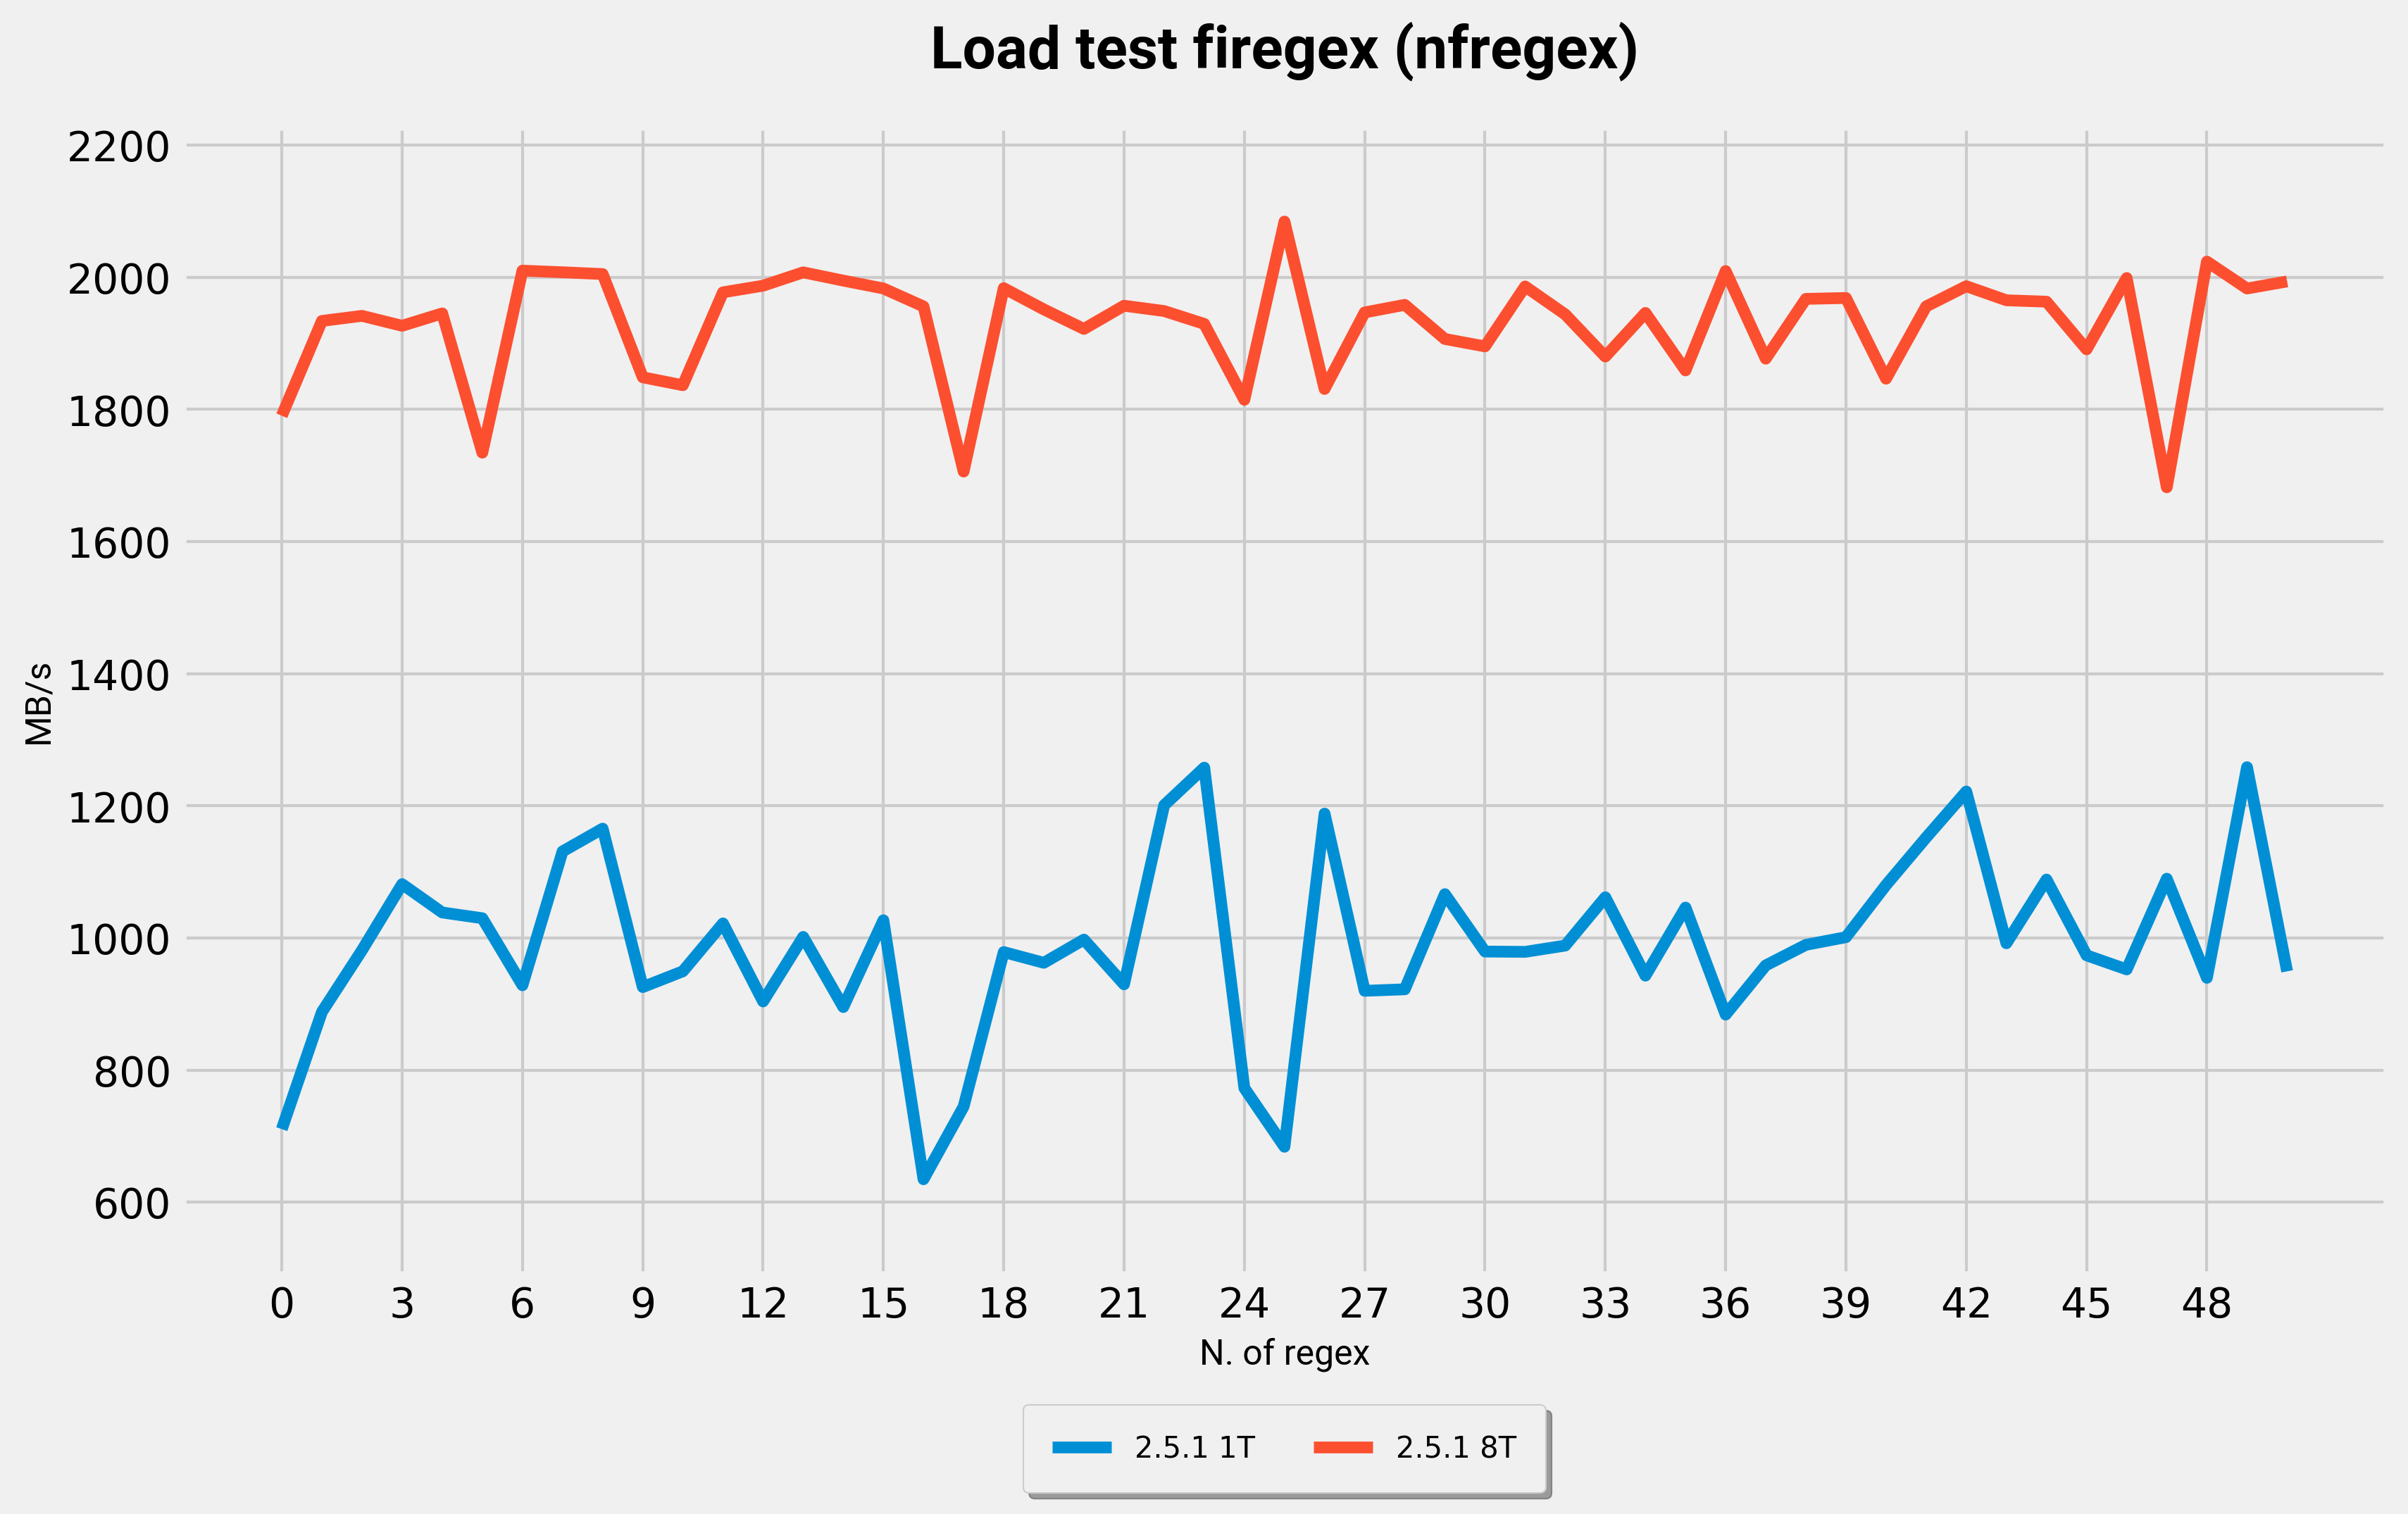
\includegraphics[width=0.98\textwidth]{images/chapter3/Benchmark-chart-with-load.png}
    \caption{NfProxy Benchmarks con load balancing personalizzato con 1 e 8 thread}
    \label{fig:nfproxy_multithread_benchmark}
\end{figure}

Gli stessi benefici sono presenti in nfproxy, infatti la base di codice per il bilanciamento dei pacchetti e la medesima per entrambi i moduli.

\section{Parsing dei pacchetti L3}

Arrivati i pacchetti nella nfqueue, questi vengono immediatamente analizzati per determinare il protocollo di livello 3,
che viene manualmente verificato tramite l'analisi dei primi 4 bit che rappresentano sia in IPv4 e in IPv6 il campo \texttt{version}.
Una volta determinata la versione del protocollo, il pacchetti viene passato ai parser per i relativi protocolli di \texttt{libtins}\footcite{\url{https://libtins.github.io/}}{libtins}.
Libtins ricorsivamente analizza i layer successivi, e ci permette di calcolare in maniera automatica lo \texttt{stream\_id},
un tipo di dato implementato nella libreria in grado di rappresentare univocamente una connessione tarmite ip e porta sorgente e destinazione in maniera ordinata:
l'ordinamento avviene prendendo la tupla ip:porta relavtivi allo stesso host come un unico valore, ed è poi l'intera tupla che veine ordinata
(se avessimo ordinato ip e porta non considerandoli a coppie, avremmo un identificativo che potrebbe essere facilmente soggetto a conflitti e per fino soggetto a
possibili attacchi al fine di bypassare i filtri del firewall stesso).
L' ordinamento permette di mantenere lo stesso identificativo sia per i pacchetti in ingresso che per i pacchetti in uscita, e dell'utilizzo di questo
dato in strutture dati come le \texttt{map}\footcite{\url{https://en.cppreference.com/w/cpp/container/map}}{std_map} utilizzate per memorizzare gli stati dei flussi.\\

\begin{listing}[H]
    \begin{minted}[
        frame=single,
        framerule=0.8pt,
        fontsize=\footnotesize,
        breaklines
      ]{cpp}
//Costruttore di PktRequest: classe che rappresenta un pacchetto effettivamente scambiata tra produttori e consumatori
PktRequest(const char* payload, size_t plen, T* ctx, mnl_socket* nl, nfgenmsg *nfg, nfqnl_msg_packet_hdr *ph, bool is_input):
    ctx(ctx), nl(nl), res_id(nfg->res_id),
    packet_id(ph->packet_id), is_input(is_input),
    packet(string(payload, plen)),
    action(FilterAction::NOACTION),
    is_ipv6((payload[0] & 0xf0) == 0x60) //Controllo della versione del protocollo
{
    if (is_ipv6){
        ipv6 = new Tins::IPv6((uint8_t*)packet.c_str(), plen); //Parsing IPv6
        sid = stream_id::make_identifier(*ipv6); // calcolo stream_id
        _original_size = ipv6->size();
    }else{
        ipv4 = new Tins::IP((uint8_t*)packet.c_str(), plen); //Parsing IPv4
        sid = stream_id::make_identifier(*ipv4); // calcolo stream_id
        _original_size = ipv4->size();
    }
    l4_proto = fill_l4_info(); // Analisi del layer di trasporto
}
\end{minted}
\end{listing}

Inoltre questo tipo di dato è agnostico rispetto al protocollo di livello 3, e pertanto può essere usato anche per un traffico misto IPv4 e IPv6, che attualmente
non è previsto per le regole e il funzionamento imposto nella fase di "inserimento" della queue nella coda di traffico, poichè ne verifichiamo che il protocollo
sia lo stesso, ma che sarebbe possibile tramite le tables L3 agnostiche di nftables, o anche semplicemente intercettando il traffico tramite diverse regole alla stessa queue,
o perfino se intercettato tramite il nome di un'interfaccia di rete che gestisce diversi indirizzzi IP, anche di versioni L3 differenti.\\
Avendo memoria condivisa, nel passaggio tra produttore e consumatore, l'analisi del pacchetto non viene persa, poichè nel passaggio del pacchetto, viene rilasciato l'indirizzo
di memoria all'oggetto c++ che rappresenta il pacchetto, la responsabilità di deallocare questa area di memoria passa al consumatore che quindi non dovrà
analizzare nuovamente il pacchetto, ma potrà direttamente procedere con la sua elaborazione.

\section{Gestione dei pacchetti TCP}

Come citato precedentemete, prima di inizializzare la queue, vengono inseriti tramite nftables le regole per intercettare il traffico in un certo punto della catena
di netfilter, per essere mandato alla queue che determinerà un verdetto sul pacchetto.\\

\begin{figure}[H]
    \centering
    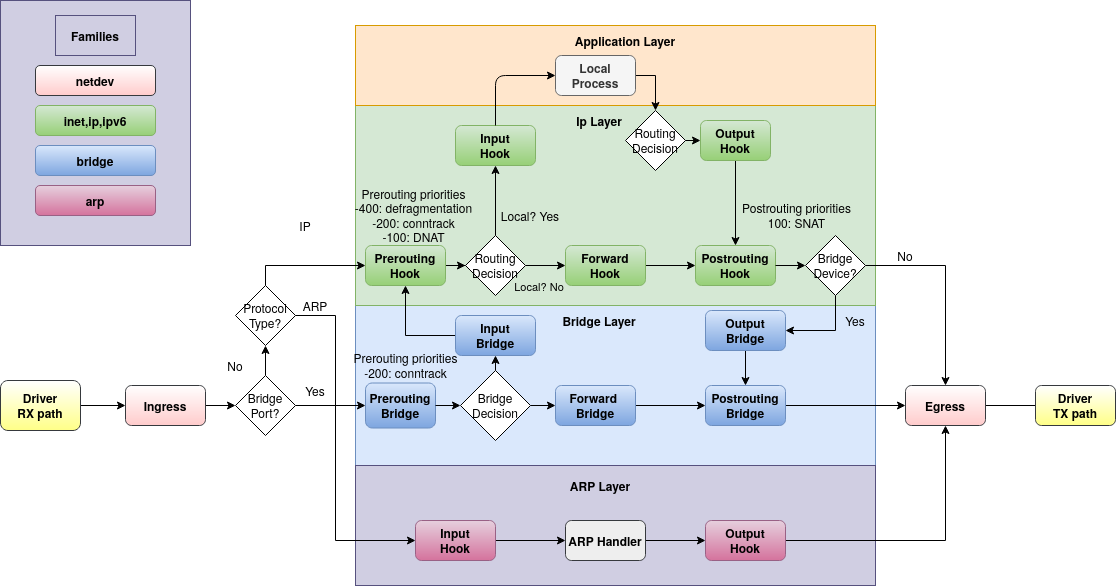
\includegraphics[width=0.98\textwidth]{images/chapter3/nf-hooks.png}
    \caption{NfTables Hooks}
    \label{fig:nftables_hooks}
\end{figure}

Il traffico in particolare viene intercettato sia in \texttt{pre-routing}, che in \texttt{post-ruoting} ad un hook prima dell'azione del modulo conntrack, ma dopo
dell'azione di defrag, in particolare a prio -310 che rientra in questo range come riportato sulla \texttt{wiki ufficiale di nftables}\footcite{\url{https://wiki.nftables.org/wiki-nftables/index.php/Netfilter_hooks}}{netfilter_hooks}.
Questo permette di ottenere dei pacchetti che hanno già subito il processo di deframmentazione a livello 3, di cui pertanto non ci dovremo preoccupare,
che non hanno subito il processo di routing (che quindi volendo potremmo manipolare) e che non sono stati ancora analizzati dal modulo conntrack.\\
Tuttavia i pacchetti non hanno subito il processo di ordinamento dei payload che avviene a livello 4, sul quale come è possibile osservare dal precedente seguente schema, non è possibile
intercettare del traffico, poichè i pacchetti arriveranno direttamente alle fasi di gestioni dei dati per la loro consegna alla socket a livello applicatvo.\\
Pertanto è dato a noi il compito di analizzare il traffico e di ordinare i pacchetti TCP per un'analisi dei dati coerente con ciò che sarà letto
dall'applicazione.\\
Fortunatamente, libtins ci permette di fare ciò in maniera automatica, e ha una gestione sufficientemente efficiente sullo scadere dei flussi TCP, sulla gestione dei buffer
e sulle problematiche di segmenti non ordinto dei pacchetti, che solleva l'applicativo da un numero importante di problematiche che andrebbero gestiste
manualmente, ma che ci vengono già gestiste nell'analisi stessa dei flussi TCP\footnote{Esempio TCP Follower: \url{https://libtins.github.io/examples/http-requests/}}.\\
Oltre al contesto creato all'interno dell'oggetto follower di libtins, viene creato uno stato esternamente per lo stesso flusso, per la memorizzatione
dello stato del flusso memorizzato con python, deallocato e allocato in maniera coerente al follower stesso, che tramite delle callback ci permette di
richiamare le azioni da eseguire sui dati che allochiamo.\\
Da notare che avremo un follower per ogni processo consumatore che analizzerà una sotto parte dei flussi dell'intero traffico, l'hashing ci garantisce che
lo stesso flusso verrà analizzato dallo stesso processo consumatore.
Anche il TCP follower è agnostico rispetto al protocollo di livello 3, e pertanto può essere utilizzato anch'esso per un traffico misto IPv4 e IPv6.

\section{Modifica dei pacchetti}

Descrizione della modifica dei pacchetti e delle problematiche riscontrate

\subsection{Traduzione di ack e seq}

Descrizione della traduzione di ack e seq

\subsection{Modifica di segmenti non ordinati}

Descrizione del problema dei segmenti non ordinati con elenco dei problemi e proposta di soluzione.
Motivazione per l'incompletezza della soluzione.

- Riferimento agli sviluppi futuri

\section{Parsing dei pacchetti HTTP}

Descrizione del parsing dei pacchetti HTTP e delle problematiche riscontrate

Riferimento all'RFC

- \url{https://github.com/domysh/pyllhttp}

\subsection{Supporto agli algoritmi di compressione HTTP}

Riferimento all'RFC

- \url{https://github.com/domysh/brotli}

- \url{https://github.com/domysh/python-zstd}
    
\subsection{Supporto alle websocket}

Descrizione del supporto alle websocket

- \url{https://websockets.readthedocs.io/en/stable/}

\section{Sintassi e gestione dei filtri python}

Gestione dei dati, e sintassi adottata per la scrittura dei filtri

\subsection{Gestione dei buffer di memoria}

Descrizione della gestione sull' 'accumulo' dei buffer in memoria

\subsection{Gestione di encoding errati}

Descrizioni delle opzioni di gestione degli encoding errati

\section{Proxy di simulazione}

Descrizione del proxy di simulazione (comando fgex)
